\chapter{Návrh}
\label{kap:navrh}

V tejto kapitole podrobne opíšeme návrh nášho riešenia autonómneho agenta pre hru Trackmania. Cieľom je vytvoriť systém, ktorý dokáže samostatne prechádzať pretekárske trate bez potreby ľudského zásahu, s dôrazom na presnosť a rýchlosť odozvy. Zameriame sa na existujúce riešenia problematiky riadení autonómnych vozidiel primárne v hre Trackmania. Pokúsime sa identifikovať problémy a navrhnúť riešenia, ktoré by mohli problémy vylepšiť. V neposlednom rade navrhneme náš systém, ktorého implementáciu rozoberieme v nasledujúcej kapitole.

\section{Existujúce riešenia}
\label{sec:riesenia
}

V komunite Trackmanie existuje veľa videí, ktoré ukazujú konkrétnu implementáciu agenta \cite{yoshtm_youtube, linesight_rl_youtube}. Tieto videá sú väčšinou určené pre širokú verejnosť a neukazujú problematiku do hĺbky. Najväčším problémom však je, že autori týchto videí neponúkajú prístup ku kódu. Taktiež sa veľa riešení venuje starším verziám Trackmanie. Z tohto dôvodu sa viacerými implementáciami môžeme iba inšpirovať. Existujú však aj riešenia, ktoré sú verejne dostupné a problematiku preberajú do hĺbky aj so zverejneným kódom. Tieto riešenia si bližšie rozoberieme v nasledujúcich podkapitolách.

\subsection{TMLR}

TMRL je framework v programovacom jazyku Python, ktorý umožňuje trénovanie hlbokej neurónovej siete pomocou učenia posilňovaním v aplikáciách, ktoré bežia v reálnom čase. Tento framework je určený pre autonómne riadenie vozidiel, ktoré z detektorov dostávajú vizuálnu informáciu o svojom prostredí. Okrem iného projekt ponúka čítateľnú implementáciu pre hru Trackmania 2020 \cite{tmrl_github}.

Na trénovanie hlbokej neurónovej siete agenta je možné použiť viacero algoritmov pre učenie posilňovaním ako Soft Actor Critic algoritmus \cite{soft_actor_critic} alebo Randomized Ensembled Double Q-Learning \cite{randomized_q_learning}. Funkcia odmeny (reward function), pomocou ktorej sa agent trénuje, sa spolieha na predpokladanú trajektóriu vozidla, ktorá musí byť najskôr odjazdená človekom. Podľa tejto predpokladanej trajektórie agent sleduje svoj progres na mape a trajektóriu vylepšuje \cite{tmrl_github}.

TMLR nám ponúka dobrú kostru na trénovanie agenta v prostredí Trackmanie a ukazuje nám problematiku, ktorú budeme musieť riešiť. Veľkou výhodou TMRL je oficiálny plugin do hry Trackmanie, ktorý neustále posiela živé dáta z hry pomocou TCP/IP spojenia na lokálnej úrovni. Implementácia má však svoje chyby, ako napríklad spoliehanie sa na ľudskú interakciu alebo na extrakciu lidar senzorov zo snímkov obrazovky hry. Agent by mal fungovať bez potrebnej ľudskej interakcie, teda by nemalo
byť potrebné aby človek ukázal približnú stopu trate a následne ju agent optimalizoval.
Taktiež extrakcia LiDAR senzorov z pixelov je zbytočne výpočtovo neefektívna a môže byť chybná \cite{tmrl_github}.


\subsection{Trackmania AI}

Trackmania AI je projekt od autora AndrejGobeX, ktorý postupne tvoril a vylepšoval agenta do počítačovej hry Trackmania. Tento projekt si prešiel vývojom od jednoduchých riešení s učením pod dohľadom až po pokročilejšie riešenia, kde sa využívalo učenie posilňovaním. Jedná sa o komplexný projekt s bohatou históriou vývoja, ktorým sa môžeme silno inšpirovať pri riešení danej problematiky \cite{trackmania_ai_github}.

Prvotné riešenia sa spoliehali na učenie pod dohľadom a na fakt, že cesta má bledošedú farbu, zatiaľčo okraje cesty mali farbu čiernu. Z tohto dôvodu sme dokázali snímku obrazovky prekonvertovať na binárnu maticu, kde boli zvýraznené bariéry cesty. Na správne rozhodnutia agenta slúžila hlboká konvolučná neurónová sieť na ktorej vstup sme posielali spomínanú binárnu maticu veľkosti 64x64 . Po konvolučných vrstvách sme do neurónovej vrstvy prireťazili aj informácie o vozidle ako je rýchlosť alebo smer. Toto riešenie malo nevýhodu v reakčnom čase. Trvalo viac ako 150 ms, kým agent pozoroval prostredie, prekonvertoval obrázok na binárnu maticu a vypočítal sa výstup neurónovej siete a vykonala sa akcia v prostredí. Z tohto dôvodu agent v tak dynamickej hre, ako je Trackmania. nestihol dostatočne rýchlo reagovať. Autor tieto problémy identifikoval a pokúsil sa ich vyriešiť \cite{trackmania_ai_github}.

Namiesto konvertovania snímky obrazovky na binárnu maticu, vyskúšal vyslať \(N\) paralelných lúčov v snímke obrazovky. Pixel po pixeli tento lúč pokračoval, až kým nenarazil na tmavý pixel. Následne sa do neurónovej siete posielalo iba \(N\) vzdialeností s rýchlosťou vozidla. Aj keď výpočet výstupu neurónovej siete bol výrazne urýchlený, počítanie lúčov zo snímky obrazovky je časovo veľmi neefektívne. Posledným vylepšením opisu prostredia zo strany autora bol radikálny krok, keď prestal prostredie sledovať pomocou snímkov z hry. Namiesto toho autor vytvoril virtuálnu dvojrozmernú mapu, v ktorej sa ku bariéram trate správal ako ku priamkam, či kružnicovým výsekom. Takýmto spôsobom môžeme pomocou geometrických výpočtov prieniku dvoch priamok alebo prieniku priamky a kružnice vypočítať vzdialenosti lúčov rôznymi smermi rýchlo a efektívne \cite{trackmania_ai_github}.


Následne autor s daným popisom prostredia implementoval učenie posilňovaním namiesto učenia pod dohľadom. Tento prístup sa vyplatil, keďže nová implementácia agenta dosahovala lepšie časy ako predošlé verzie. Tento agent nebol však dokonalý, keďže na testovacej trati bol stále pomalší ako skúsený hráč. Hráč na rozdiel od agenta dokáže trať prechádzať viackrát a pamätať si postupnosť zákrut, ktoré nasledujú. V tejto implementácii agent vidí iba aktuálnu lokálnu informáciu a vôbec nevie, aké zákruty ho čakajú \cite{trackmania_ai_github}.



\subsection{Gran Turismo Sophy AI}

Gran Turismo Sophy AI je pokročilý projekt spoločností Sony AI, Polyphony Digital a Sony Interactive Entertainment, ktorý sa zameriava na vytvorenie autonómneho agenta schopného dosahovať nadľudské výkony v závodnej hre Gran Turismo \cite{sophy_ai}. Súčasťou tohto projektu je aj práca \textit{Super-Human Performance in Gran Turismo Sport Using Deep Reinforcement Learning} \cite{super_human_grand_turismo}, ktorá podrobne opisuje techniky a metódy použité na trénovanie tohto agenta.

V tejto práci dosahoval agent nadľudské výkony tým, že využíval pokročilé metódy hlbokého posilňovaného učenia. Na rozdiel od tradičných prístupov nebolo potrebné používať snímky obrazovky na sledovanie prostredia. Namiesto toho agent využíval analógiu LiDAR senzorom, a globálne informácie o trati, ako napríklad nadchádzajúce zákruty a ich poradie. \cite{super_human_grand_turismo}.

Práca \textit{Improving Trackmania Reinforcement Learning Performance: A Comparison of Sophy and Trackmania AI} \cite{imporving_trackmania_AI} sa pokúša aplikovať a vylepšiť tieto metódy v spomínanom projekte Trackmania AI. Autor sa snažil implementovať zlepšenia na princípe Sophy AI, pričom sa zameriaval na použitie podobných techník pre zvýšenie výkonu agenta v hre Trackmania.


%%  ===========================================================================================

\section{Problémy a navrhované riešenia}
\label{sec
}

V predchádzajúcej podkapitole sme mohli vidieť rôzne prístupy a implementácie agentov do pretekárskych hier. Obe implementácie agentov v hre Trackmania mali svoje nedostatky. Pokúsime sa identifikovať hlavné problémy a prekážky, ktoré budeme musieť vyriešiť v našej implementácii a navrhnúť potrebné riešenia.

\subsection{Pomalá odozva}
Pri riešeniach, v ktorých sme na opis prostredia používali snímku obrazovky alebo sme zo snímky obrazovky extrahovali údaje podobné LiDAR senzorom, sme sa mohli stretnúť s nízkou odozvou. Tento problém spočíva v tom, že hra beží vo full HD rozlíšení, pričom spracovanie takého obrazu je výpočtovo náročné a drahé na čas. Pri dynamickej hre ako Trackmania potrebujeme, aby agent na zmeny v prostredí reagoval čo najrýchlejšie. V ideálnom prípade by agent mal vedieť reagovať do 10 ms, čo je čas, za ktorý sa aktualizuje herný engine Trackmanie.

Aj napriek tomu, že hráč na hranie hry potrebuje iba obraz z hry, mali by sme sa zamyslieť aj nad iným prístupom pre nášho agenta. Na zlepšenie pomalej odozvy by bolo vhodné úplne eliminovať aspekt počítačového videnia a spracovania obrazu. Je potrebné si uvedomiť, že Sophy AI dosahuje nadľudské výsledky bez toho, aby graficky videlo samotnú hru. Namiesto snímkov obrazovky agent dostáva vzdialenosti k okrajom trate, čo je analógia k LiDAR senzorom \cite{sophy_ai, super_human_grand_turismo}.

\begin{figure}
\centerline{\includegraphics[width=0.6\textwidth]{images/LiDAR_raycast.png}}
%popis obrazku
\caption[LiDAR senzor]{Na obrázku je prezentovaná simulácia LiDAR senzora, ktorá by mohla poslúžiť ako alternatíva k počítačovému videniu v našej implementácii.
}
\label{obr:LiDAR}
\end{figure}


\subsection{Závislosť na ľudskej interakcii}
Implementácie ako TMLR sa spoliehajú na nahranie orientačnej dráhy človekom. Následne agent sleduje svoj progres na trati vzhľadom k tejto trajektórii. Bez človeka by agent nebol schopný prejsť trať, čím agent stráca autonómnosť \cite{tmrl_github}.

Tento problém by sme dokázali vyriešiť tak, že namiesto nahrania orientačnej trajektórie prehľadáme priestor mapy a nájdeme cestu zo štartu do cieľa.

\subsection{Limitácia človekom}
Výhodou implementácie, ktorá bola založená na učení pod dohľadom (supervised learning), bola jednoduchosť a kvalita dosiahnutých výsledkov vzhľadom na čas strávený samotným trénovaním neurónovej siete. Pre zlepšenie spoľahlivosti a rýchlosti agenta trénovaného pod dohľadom je potrebný podstatne väčší dataset a lepší hráč \cite{trackmania_ai_github}. Tento problém by sme mohli vyriešiť extrakciou dát zo záznamov najrýchlejších hráčov na ľubovoľnej mape. Takýto prístup je však stále obmedzený ľudským faktorom, keďže podľa definície učenia pod dohľadom agent nikdy nebude lepší ako človek, ktorý poskytol trénovacie dáta \cite{artificial_intelligence_modern_aproach}.

Na riešenie tohto problému by sme mali namiesto učenia pod dohľadom použiť učenie posilňovaním, čím agenta nebudeme limitovať a teoreticky by mohol byť schopný nadľudských výkonov, ako sme mohli vidieť v prípade Sophy AI \cite{sophy_ai, super_human_grand_turismo}.

\subsection{Neznalosť trate}
V bežných podmienkach má hráč Trackmanie možnosť opakovane absolvovať danú mapu, čo mu umožňuje získať znalosť trate a zapamätať si postupnosť zákrut. Toto opakovanie je predovšetkým dôležité vzhľadom na skutočnosť, že pre rovnakú zákrutu môže existovať viacero ideálnych trajektórií, ktoré závisia od nasledujúceho úseku za danou zákrutou. Ak za zákrutou nasleduje ďalšia ostrá zákruta, cieľom je prejsť prvú zákrutu tak, aby sa vytvoril vhodný vstup do druhej zákruty. V prípade, že za zákrutou nasleduje rovina, je žiadané prejsť zákrutou s čo najväčšou rýchlosťou, aby sa minimalizovala časová strata na dlhej rovine.

Problémom oboch implementácií TMRL a Trackmania AI je fakt, že agent pri rozhodovaní používa iba lokálnu informáciu a nemá celkový prehľad o širšom kontexte. Pod pojmom lokálna informácia môžeme chápať iba aktuálnu snímku obrazovky alebo aktuálny stav LiDAR senzorov. Aj keď sa snažíme tento problém čiastočne riešiť pridaním informácií o vozidle ako je napríklad rýchlosť, agent stále nie je schopný plánovať kroky dostatočne dopredu na rozdiel od hráča, ktorý má možnosť trať hrať opakovane \cite{tmrl_github, trackmania_ai_github}.

Riešenie problému, okrem poskytnutiu lokálnych informácií o agentovom okolí a stave vozidla, ako je rýchlosť a smer, pridať aj opis trate v nasledujúcom úseku, napríklad niekoľko nasledujúcich bodov stredovej osi trate, ako je realizované v spomínanej práci \cite{super_human_grand_turismo}. Týmto spôsobom poskytneme agentovi viac informácií o budúcich zákrutách, čo pomôže agentovi v lepšom plánovaní trajektórie a iba minimálne zväčší rozmer dát agentových senzorov \cite{super_human_grand_turismo}.


\begin{figure}
\centerline{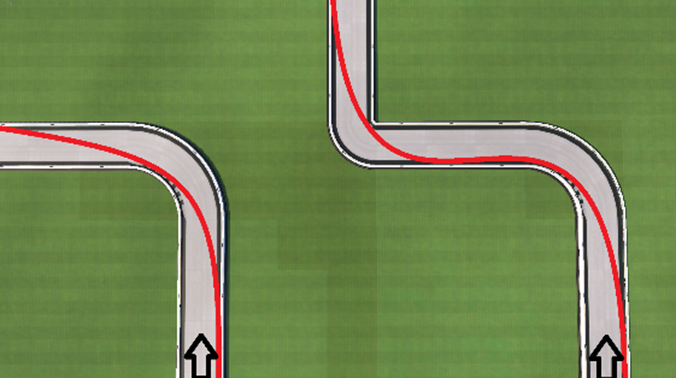
\includegraphics[width=0.6\textwidth]{images/trajectory.png}}
%popis obrazku
\caption[Optimálna trajektória]{Na obrázku sú zobrazené dve odlišné cesty, ktoré majú spoločnú prvú zákrutu, ale líšia sa v úseku za touto zákrutou. Je viditeľná variabilita optimálnych trajektórií pre tieto cesty.
}
\label{obr:trajectory}
\end{figure}


\begin{figure}
\centerline{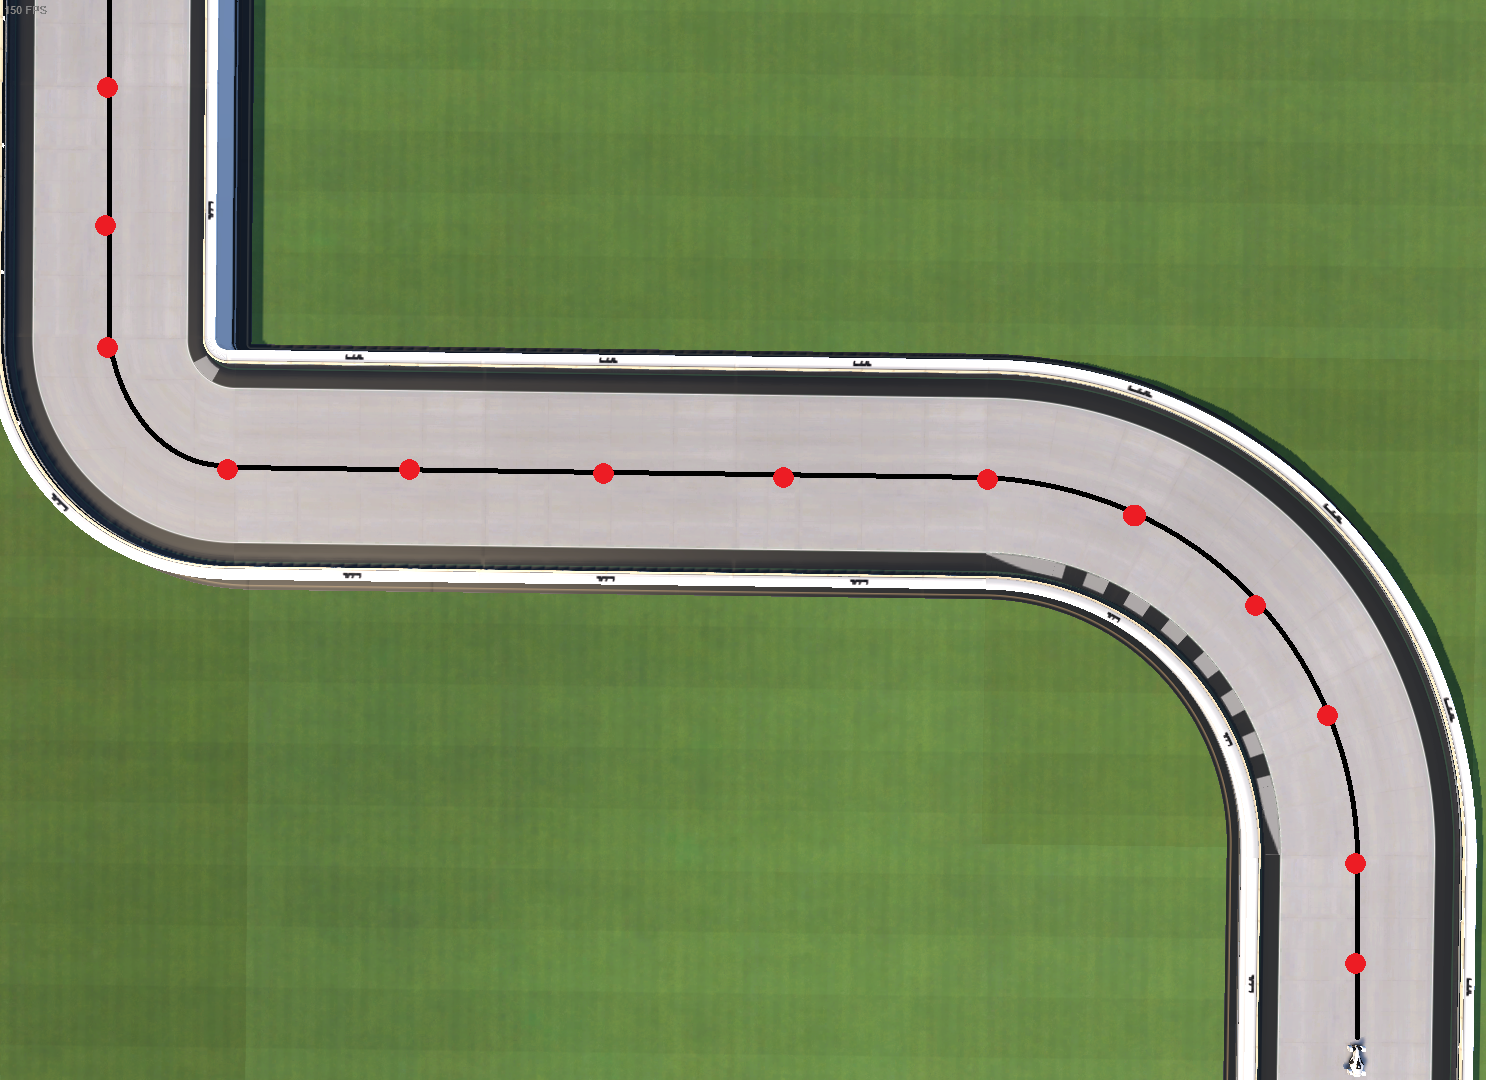
\includegraphics[width=0.6\textwidth]{images/steering_theory.png}}
%popis obrazku
\caption[Globálna informácia trate]{Na obrázku sú červenou farbou znázornené body, ktoré ležia na stredovej osi trate. Táto informácia by poskytla agentovi lepší pojem o prostredí.
}
\label{obr:steering}
\end{figure}

\subsection{Nevšeobecnosť riešenia}
Autor v práci Trackmania AI správne identifikoval problémy so zlou odozvou. Tento problém sa pokúsil odstrániť eliminovaním aspektu počítačového videnia a spracovania obrazu. Vytvoril teda model mapy pomocou priamok a polkruhov. V tomto modeli mohol následne rýchlo a efektívne počítať vzdialenosti auta od bariér trate pomocou geometrických výpočtov (prienik dvoch priamok, prienik priamky a roviny). Aj napriek tomu, že toto riešenie je veľmi rýchle a elegantné, v budúcnosti by nebolo možné agenta vylepšiť, aby sa dokázal pohybovať aj po mape s výškovým prevýšením alebo slučkami v mape.

Na riešenie tohto problému by sme mohli ostať pri podobnej myšlienke, avšak namiesto 2D modelu mapy by sme vytvorili 3D model mapy. Takýto prístup by nám umožnil simulácie na tratiach, ktoré obsahujú výškové prevýšenia alebo slučky, pričom by sme nestratili výhodu využitia efektívnych geometrických výpočtov na základe simulácie LiDAR senzorov. Odstránením limitácie roviny ako priestoru by sme simuláciu viac priblížili k realite \cite{trackmania_ai_github}.




\section{Návrh agenta}

Aby sme správne navrhli agenta, potrebujeme jasne popísať problematiku, ktorú budeme riešiť tak, ako sme ukázali v podkapitole \ref{sec:umela_inteligencia}.

\subsection{Typ agenta a prostredie}

Našou úlohou je implementovať šoféra, ktorý bude vedieť plne autonómne prejsť jednoduchú trať v počítačovej hre Trackmania. Nášho agenta budeme považovať za racionálneho, ak bude vedieť odjazdiť trať od štartu až po cieľ. Taktiež budeme vedieť agenta hodnotiť podľa výsledného času, teda úlohou agenta bude minimalizovať čas prejdenia trate.

\subsection{Senzory}

Z problematiky existujúcich riešení nám vyplýva, že by sme sa chceli vyhnúť spracovaniu obrazových dát a namiesto toho bude agent svoje prostredie vnímať pomocou simulácie LiDAR senzorov. LiDAR senzory vieme najreálnejšie simulovať pomocou počítačovej grafiky a techniky raycastingu. Bude potrebné vytvoriť 3D model trate, v ktorom budeme následne vysielať lúče z pozície auta rôznymi smermi podľa otočenia auta. Tieto lúče môžeme matematicky popísať nasledovne:

\begin{equation}
\text{distance}_i = \min_{t \geq 0} \{ t : \mathbf{r}(t) \cap \text{mesh} \neq \emptyset \}
\end{equation}

kde $\mathbf{r}(t) = \mathbf{p}_0 + t \mathbf{d}_i$ je parametrická rovnica lúča vyslaného z počiatočnej pozície auta $\mathbf{p}_0$ v smere $\mathbf{d}_i$, a $\text{mesh}$ reprezentuje 3D model prostredia. Hľadáme najmenšie $t \geq 0$, pri ktorom lúč $\mathbf{r}(t)$ pretne model trate. Týmto spôsobom vieme určiť vzdialenosť prekážok v rôznych smeroch okolo auta.

Okrem tejto lokálnej informácie bude mať agent prístup aj ku globálnej informácii, ako vyzerajú nasledujúce zákruty či roviny. Taktiež agent bude mať k dispozícii údaje o stave vozidla, ako sú rýchlosť, pozícia auta na mape alebo smer auta \cite{reinforcment_in_real_time, artificial_intelligence_modern_aproach}.

\subsection{Efektory}

Agent bude ovládať formulu pomocou simulácie ľudskej interakcie s počítačom. Tu si môžeme uvedomiť, že auto v Trackmánii môžeme ovládať dvomi spôsobmi a to pomocou klávesnice alebo analógového ovládača.

\begin{itemize}
\item \textbf{Klávesnica} umožňuje ovládanie vozidla pomocou štyroch kláves, napríklad šípok, ktoré môžeme stláčať nezávisle. Výhodou tohto prístupu je jednoduchosť, keďže každá šípka môže byť zapnutá alebo vypnutá, existuje $2^4$ možných kombinácií kláves, pričom nie každá kombinácia bude validná. Nevýhodou tohto prístupu je, že ak by agent chcel zatočiť iba mierne, naša implementácia by mu to neumožnila. Môžeme sa stretnúť s problémami, keď by agent mohol naraziť, pretože sme mu nedovolili jemne meniť smer vozidla.

\item \textbf{Analógový ovládač} nám umožňuje ovládať vozidlo pomocou dvoch binárnych páčok, ktoré predstavujú plyn a brzdu. Plyn aj brzda môžu byť buď zapnuté alebo vypnuté. Otočenie kolies realizujeme pomocou analógovej páčky, ktorej hodnotu môžeme reprezentovať ako reálne číslo v rozsahu [-1, 1]. Výhodou tohto prístupu je, že agent bude mať možnosť rozhodovať aj o jemnejšej korekcii pohybu, ako je zobrazené na obrázku \ref{obr:controler_keyboard}, kde vozidlo zatáča len o 34\%. Agent nie je obmedzený na binárne ovládanie vozidla, čo vedie k lepšej kontrole. Nevýhodou tohto prístupu je výrazne väčší akčný priestor, keďže sme z diskrétneho priestoru prešli do spojitého priestoru.
\end{itemize}

\begin{figure}

\centerline{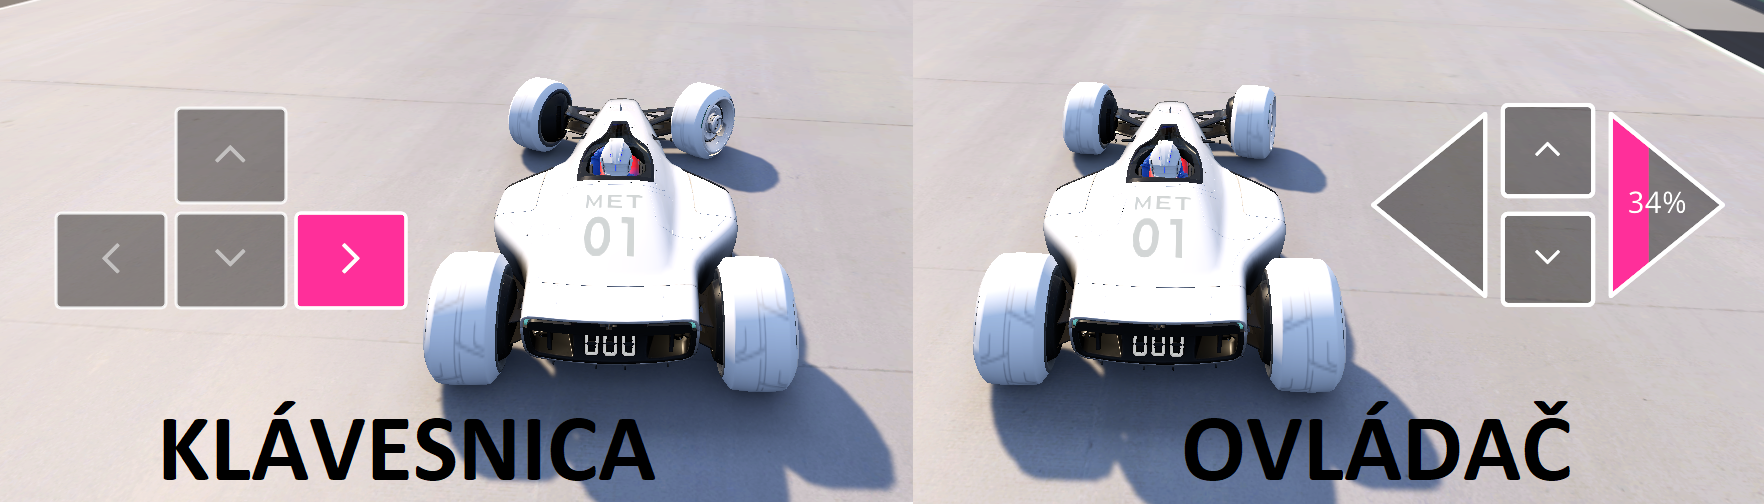
\includegraphics[width=1\textwidth]{images/kayboard_controller.png}}
%popis obrazku
\caption[Rozdiel ovládania]{Obrázok ilustruje výhodu použitia ovládača vďaka jeho schopnosti jemného ovládania a presnosti pohybu.}

\label{obr:controler_keyboard}
\end{figure}
 

Pre jemnejšie ovládanie vozidla sa v našom prípade rozhodneme pracovať s analógovým ovládačom, aby mal agent lepšiu a citlivejšiu kontrolu nad vykonávanými akciami.

\subsection{Rozhodovacia funkcia agenta}

V podkapitole \ref{sec:umela_inteligencia} sme popísali, že agent je formálne definovaný ako funkcia, ktorá zobrazuje postupnosť vnemov na požadovanú akciu. Rozhodovacia funkcia agenta by teda mohla byť popísaná ako tabuľka vnemov a výstupov, v ktorej by sme hľadali akú akciu máme v danom momente vykonať. Táto tabuľka by bola však nekonečne veľká a vždy by sme dokázali agenta dostať do situácie, v ktorej sa ešte nenachádzal, keďže agent sa pohybuje v spojitom prostredí.

Vieme, že rozhodovacia funkcia agenta môže byť teda aj obyčajná funkcia s podmienkami. Ak by sme však mali vytvoriť takúto funkciu, v ktorej by sme sa snažili popísať za akých podmienok má agent vykonať akú akciu, prišli by sme na to, že je to nemožné, keďže agent sa pohybuje vo spojitom svete a akcie sme určili tiež ako spojitý priestor. Využijeme teda základnú vlastnosť neurónových sietí, ktorá nám hovorí o tom, že neurónová sieť dokáže aproximovať ľubovoľnú funkciu \cite{artificial_intelligence_modern_aproach}. Na rozhodovanie agenta teda použijeme hlbokú neurónovú sieť, ktorá bude aproximovať funkciu agenta, teda bude zobrazovať vnemy na akcie.

Vstupná vrstva do neurónovej siete bude mať rozmer \(N + M + 6\). Táto sieť bude na vstupe očakávať nasledovné údaje: \(N\)-rozmerný vektor vzdialeností k prekážkam získaný simuláciou LiDAR senzora, \(M\)-rozmerný vektor nasledujúcich inštrukcií zákrut na mape (zákruty doľava majú zápornú hodnotu, zákruty doprava kladnú hodnotu, rovné úseky majú hodnotu 0; čím ostrejšia zákruta, tým je číslo ďalej od nuly), rýchlosť vozidla v smere jeho pohybu, rýchlosť vozidla v smere kolmého na smer pohybu, uhol medzi predným vektorom vozidla a orientačnou dráhou trate a predchádzajúcu akciu (3 hodnoty). Výstupná vrstva bude mať rozmer 3, obsahujúci akcie pre plyn, brzdu a zatáčanie.


\subsection{Trénovanie neurónovej siete}
Na upravenie váh neurónovej siete môžno použiť niekoľko techník. 

\begin{itemize}
    \item {\textbf{Učenie pod dohľadom: }
        V tomto prípade by sme potrebovali získavať dáta hraním hry, pričom by sme ukladali stav senzorov s požadovanými akciami. Následne by sme z týchto dát mohli natrénovať našu neurónovú sieť. Výhodou tohto prístupu by bola jednoduchosť riešenia. Problémom by mohlo byť získanie dostatočného množstva dát. Taktiež by sme sa obmedzili na ľudskú interakciu a agent by podľa definície šoféroval v najlepšom prípade tak dobre, ako človek, ktorý ho trénoval.
    }

    \item {\textbf{Učenie posilňovaním:} Učenie posilňovaním (reinforcement learning) dobre zrkadlí definíciu agenta interagujúceho s prostredím a je pri trénovaní autonómnych vozidiel často využívaným prístupom. Tento prístup nám umožňuje experimentovať s rôznymi odmeňovacími funkciami, čo z neho robí vhodnú voľbu pre náš projekt.}

    \item {\textbf{Evolučný algoritmus:} Na trénovanie neurónovej siete, ktorá by slúžila na rozhodovanie o akciách agenta, by sa dal použiť genetický algoritmus NEAT (NeuroEvolution of Augmenting Topologies) \cite{neat_article}. Tento algoritmus vyžaduje niekoľko jedincov, ktorí by sa medzi sebou krížili, avšak Trackmania nám umožňuje mať otvorenú iba jednu inštanciu hry. Tento prístup by bol teda veľmi zdĺhavý, keďže by sme kvalitu jedincov nemohli testovať naraz, ale postupne, pričom kvalita výsledkov nie je zaručená.}

\end{itemize}

\section{Predpoklady a obmedzenia}

Riadenie vozidla v hre Trackmania je veľmi náročný problém. Autor v práci \cite{trackmania_is_np}
opisuje, že iba rozhodovanie sa o poradí, v akom pozbierame kontrolné body je, NP-ťažký problém, teda ho nedokážeme riešiť v polynomiálnej časovej zložitosti. Okrem toho sa v Trackmánii môžu vyskytovať rôzne povrchy a stovky odlišných blokov, čo nám umožnuje vytvárať obrovské množstvo tratí. Práve kvôli týmto dôvodom si budeme musieť problém zjednodušiť a určiť niekoľko predpokladov.


\begin{itemize}
    \item {
        Mapa sa bude skladať iba z jednoduchých asfaltových blokov, ako sú roviny, zákruty, štart, cieľ a kontrolná brána. 
    }
    \item {
        Dráha nebude obsahovať žiadne výškové prevýšenie a bude postavená iba v jednej rovine, aby sme sa vyhli skokom.
    }

    \item {
        Na trati sa nebudú nachádzať žiadne križovatky a bloky trate budú na seba nadväzovať podobne ako spájaný zoznam. Takýmto spôsobom budeme vedieť určiť orientačnú dráhu bez ľudského zásahu. Riešenie takého problému, kedy by sme sa snažili hľadať aj najoptimálnejšiu cestu, je nad rámec tejto práce, keďže najkratšia cesta nemusí byť nutne najrýchlejšia pre pretekárske auto. V špecifických prípadoch by sa nám oplatilo uprednostniť dlhšiu cestu, ktorú by sme vedeli prejsť vyššou rýchlosťou.
    }
\end{itemize}








